\documentclass[../main.tex]{subfiles}

\newcommand{\rot}{\text{rot}}

\newcommand{\kp}{k_{+}}
\newcommand{\km}{k_{-}}
\newcommand{\kz}{k_{z}}
\newcommand{\st}{S}
\newcommand{\stp}{\overline{S}_{+}}
\newcommand{\stm}{\overline{S}_{-}}
\newcommand{\swp}{\widetilde{S}_{+}}
\newcommand{\swm}{\widetilde{S}_{-}}
\newcommand{\vep}{\varepsilon}

\begin{document}
    \chapter{Плазмонные эффекты в HgCdTe}
    
    Плазмоны - это квазичастицы, отвечающие квантованию 
    Ленгмюровских колебаний. Они в значительной мере 
    определяют оптические свойства материалов, в том числе 
    гетероструктур на основе $Hg_xCd_{1-x}Te$.

    \section{Электродинамические свойства двумерных плазмонов}

    Плазмоны представляют собой TM волны, имеющие одну компоненту 
    магнитного поля $\vec H$ и две компоненты электрического $\vec E$. 
    Они распространяются вдоль проводящего слоя. Схематичное изображение 
    электрического поля приведено на Рис. \ref{plasmons:schematic:fields}.

    \begin{figure}[h]
        \begin{minipage}[h]{1\textwidth}
            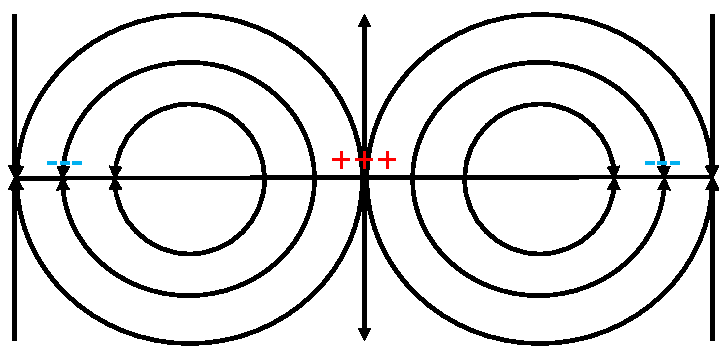
\includegraphics[width=0.7\textwidth]{./images/schematic_field.pdf}
            \caption{Схематичное изображения распределения поля плазмона.
            \label{plasmons:schematic:fields}}
        \end{minipage}
    \end{figure}

    Рассмотрим свойства плазмонов, в предположении, что ток,
    соответствующий им локализован в квантовой яме и течет только
    в плоскости. Аппроксимация $\delta$ функцией является 
    справедливой, поскольку характерная длина волны имеет порядок 
    единиц $\mu\text{m}$, a толщина квантовой ямы - порядок единиц 
    $\text{nm}$. Тогда из уравнений Максвелла:
    \begin{equation}
        \rot \vec H = \frac{\varepsilon}{c} \dot{\vec E} + \delta(z) \vec j;
    \end{equation}

    Предположим, что ток обусловлен исключительно электрическим полем
    $\vec j  = \sigma \vec E$ и сделаем предположения о направлениях 
    $\vec j \parallel \vec E \parallel \vec{x}_0, \vec H \parallel \vec{y}_0$.
    Распишем по компонентам, здесь важно отметить, что $\varepsilon$ 
    - полная диэлектрическая проницаемость:
    \begin{equation}
        \begin{aligned}
            \partial_x H_y &=& \frac{\varepsilon}{c} \dot{E}_z;
            -\partial_z H_y &=& \frac{\varepsilon}{c} \dot{E}_x + \frac{4\pi };
        \end{aligned}
    \end{equation}

    Принимая во внимание уравнение на электрическое поле:
    \begin{equation}
        \rot \vec E = \frac{1}{c} \dot \vec H;
    \end{equation}

    Сделаем Фурье преобразование электрического поля в плоскости квантовой ямы
    и получим замкнутую систему уравнений:
    \begin{equation}
        \left\{
        \begin{aligned}
            - i \frac{\omega}{c} H_y &=& i k E_z - \partial_z E_x;\\
            - \partial_z H_y  &=& \frac{4\pi}{c} \underbrace{\sigma E_x}_{\vec j} 
            - i \varepsilon  \frac{\omega}{c} E_x;\\
            ik H_y  &=& - i \varepsilon \frac{\omega}{c} E_z;
        \end{aligned}
        \right.
    \end{equation}

    Решая её получим уравнение на зависимость поля от $z$:
    \begin{equation}
        \frac{\partial^2 E_x}{\partial z^2} = \frac{4\pi i}{\varepsilon \omega}
        \underbrace{\left(k^2  - \varepsilon \frac{\omega^2}{c^2}\right)}_{q^2} \sigma E_x \delta(z)
        + \underbrace{\left(k^2  - \varepsilon \frac{\omega^2}{c^2}\right)}_{q^2} E_x;
    \end{equation}

    Предположим решение в виде спадающих от квантовой ямы экспонент
    с волновым вектором $i\alpha$:
    \begin{equation*}
        E_x = \left\{
            \begin{aligned}
                E_0 \exp{-\alpha z} & &z > 0\\
                E_0 \exp{\alpha z} & &z < 0
            \end{aligned}
        \right.;
    \end{equation*}

    Интегрируя в окрестности нуля получим граничное условие на на производные:
    \begin{equation*}
        \left.\frac{\partial E_x}{\partial z}\right\vert{}^{+0}_{-0} = \frac{4\pi i}{\varepsilon \omega}
        \left(k^2  - \varepsilon \frac{\omega^2}{c^2}\right);
    \end{equation*}

    Отсюда можно получить дисперсионное соотношение для таких двумерных плазмонов:
    \begin{equation}
        \label{plasmons:edisp}
        k^2  = \varepsilon  \frac{\omega^2}{c^2} - \left(\frac{\varepsilon\omega}{2\pi \sigma}\right)^2;
    \end{equation}



%СИСТЕМА СИ- СГС

%ПРОЯСНИТЬ значенние эпсилона 
    
    \section{Дисперсионные соотношения плазмонов}

    Поскольку речь идёт о классических ЭМ колебаний, 
    для получения дисперсионного соотношения необходимо найти 
    материальные соотношения, а в частности - зависимость 
    диэлектрической поляризуемости от частоты и волнового вектора.

%ПРОЯСНИТЬ АЛЬФУ

    Выражение для поправки к диэлектрической проницаемости является 
    обобщением т.н. формулы Линдхарда (учитывается несколько зон, в то 
    время как сам Линдхард работал в однозонном приближении)
    и приведено ниже:
    \begin{equation}
        \label{lindhard}
        \kappa_{pl}(\vec q, \omega) = \frac{4\pi}{\vec{q}^2 V}
            \sum_{m, n} \int d\vec k \frac{f_m(\vec k) - f_n(\vec k 
                + \vec q)}{\varepsilon_n(\vec k + \vec q) - 
                \varepsilon_m - \hbar \omega - \i \hbar \alpha}
                \bra{\psi_{\vec k + \vec q,n}} \ket{\psi_{\vec k, m}};
    \end{equation}

%ПРОСЯНИТЬ q ПРОЯСНИТЬ ПЕРЕМЕННЫЕ

    Ленгмюровские колебания являются колебаниями поляризации. Таким
    образом они должны подчиняться уравнению связи поляризации и 
    плотности свободного заряда $\div \vec P  = - \rho$. Кроме того 
    такие колебания могут возбуждаться внешним электрическим полем, 
    которое мы примем потенциальным $\vec E = - \grad \varphi$ и 
    гармоническим. Тогда оно будет давать добавку потенциальной энергии:
    \begin{equation}
        \label{plazmon:field}
        \hat \varphi  = U \exp{i\vec q \vec r - i \omega t}
            + U^{\dagger} \exp{-i\vec q\vec r + i \omega t};
    \end{equation}

    В общем виде функции представляются в виде огибающей, зависящей 
    от времени и быстро осциллирующего члена. В частности:
    \begin{equation}
        \label{plasmons:wf0}
        \ket{\vec k, m} = \frac{1}{\sqrt S} \exp{i\vec k \vec r}
            \exp{-i \omega_{\vec k, m} t} \psi_{\vec k, m};
    \end{equation}

    Здесь $\vec k$ - волновой вектор, которому отвечает функция, 
    $m$ - номер подзоны с учётом спина и размерного квантования 
    по оси $z$. $\psi_{\vec k, m}$ - волновые функции
    \ref{calculation:wf}, полученные по методике, 
    описанной в прошлой главе \ref{chapter:calcs}. 

    Электрическое поле в виде \ref{plazmon:field} должно вызывать 
    искажения 
    такой равновесной волновой функции с волновыми векторами
    $\vec k \pm \vec q$, т.e. в первом порядке малости по полю:
    \begin{equation}
        \label{plasmons:wf1}
        \psi_m (\vec k, \vec r) = \ket{\vec k, m} + \sum_n b_{\vec k 
            + \vec q, m, n} (t) \ket{\vec k + \vec q, n} + \sum_n 
            c_{\vec k - \vec q, m, n} (t) \ket{\vec k - \vec q, n};
    \end{equation}

    В таком случае плотность заряда может быть записана как:
    \begin{multline}
        \label{charge_density}
        \rho = -e \sum_{m} \int d\vec k  \left(
            \bra{\psi_m (\vec k, \vec r}\ket{\psi_m (\vec k, 
            \vec r} - 1\right) f_m(\vec k) =
            \sum_{m, n} \int d \vec k f_m (\vec k) \\
            \left( b_{\vec k + \vec q, m, n} (t)
            \bra{\vec k, m} \ket{\vec k 
            + \vec q, n} + b^\dagger_{\vec k + \vec q, m, n} (t) 
            \bra{\vec k + \vec q, n} \ket{\vec k, m}\right.\\ 
            \left. + c_{\vec k - \vec q, m, n} (t) \bra{\vec k, m} 
            \ket{\vec k  - \vec q, n} + c^\dagger_{\vec k - \vec q, m, n} 
            (t) \bra{\vec k - \vec q, n} \ket{\vec k, m} \right);
    \end{multline}
    
    Для получения коэффициентов $b,~c$ воспользуемся нестационарной 
    теорией возмущений.

    Результатом для вычисления коэффициентов является:
    \begin{equation}
        \label{plasmons:charge:coeffs}
        \begin{aligned}
            b_{\vec k + \vec q, m, n} (t) = U \frac{\exp{-i\omega t - i 
                \varepsilon_m (\vec k) t / \hbar + i \varepsilon_n(\vec k 
                + \vec q) t / \hbar + \alpha t}}{\varepsilon_m (\vec k) + \hbar 
                \omega - \varepsilon_n(\vec k + \vec q)+ i \hbar \alpha}
                \bra{\psi_{\vec k+\vec q, n}}\ket{\psi_{\vec k, m}}; \\
            c_{\vec k - \vec q, m, n} (t) = U^\dagger \frac{\exp{i\omega t - i 
                \varepsilon_m (\vec k) t / \hbar + i \varepsilon_n(\vec k 
                - \vec q) t / \hbar + \alpha t}}{\varepsilon_m (\vec k) - \hbar 
                \omega - \varepsilon_n(\vec k - \vec q)+ i \hbar \alpha}
                \bra{\psi_{\vec k+\vec q, n}}\ket{\psi_{\vec k, m}};
        \end{aligned}
    \end{equation}

    В частности, стоит отметить, что для случая квантовой ямы, скалярное 
    произведение функций вида $\psi_{k, m}$ будет содержать в том числе 
    и скалярное произведение по оси $z$. Предполагая квантованность по 
    этой оси:
    \begin{multline}
        \bra{\psi_{\vec q, n}}\ket{\psi_{\vec k, m}} = 
            \bra{\sum_i \exp{k_{z,i} \sum_j c_{nij \vec q}} u_j(\vec r)}
            \ket{\sum_i \exp{k_{z,i} \sum_j c_{mij \vec k}} u_j(\vec r)}\\ 
            = \sum_{s=\{i,j\}}  c^\dagger_{ns \vec q} c_{ms \vec k};
    \end{multline}

    Подставляя полученные выражения в \ref{charge_density} 
    и приводя подобные можно получить:
    \begin{multline}
        \label{charge_full}
        \rho = \frac{e^2 U}{S} \exp{i\vec q \vec r - i \omega t + \alpha t}
            \sum_{m, n} \int d\vec k \left( \frac{\bra{\psi_{\vec k + \vec q, n}}
            \ket{\psi_{\vec k, m}}}{\varepsilon_m(\vec k) + \hbar \omega - 
            \varepsilon_n(\vec k + \vec q) + i \hbar \alpha} +\right. \\ 
            \left. \frac{\bra{\psi_{\vec k - \vec q, n}}
            \ket{\psi_{\vec k, m}}}{\varepsilon_m(\vec k) - \hbar \omega - 
            \varepsilon_n(\vec k - \vec q) - i \hbar \alpha} \right) + \text{c.c.}=\\
            \frac{e^2 U}{S} \exp{i\vec q \vec r - i \omega t + \alpha t}
            \sum_{m, n} \int d\vec k \bra{\psi_{\vec k + \vec q, n}}
            \ket{\psi_{\vec k, m}} \frac{f_m(\vec k) - f_n(\vec k - \vec q)}
            {\varepsilon_m(\vec k) + \hbar \omega - \varepsilon_n(\vec k + \vec q) 
            + i \hbar \alpha};
    \end{multline}

    Учитывая это выражение мы получаем формулу Линдхарда \ref{lindhard}. Обладая 
    этим знанием сравнительно легко получить дисперсионное соотношение для плазмонов
    \ref{plasmons:edisp}, решая следующее уравнение, здесь $\kappa$ - 
    диэлектрическая проницаемость барьеров:

%ЧТО ТАКОЕ КАППА

    \begin{equation}
        \label{plasmons:disp}
        \frac{1}{(2\pi)^2}\frac{\kappa^2}{\kappa^2_{pl}} = 
        \vec{q}^2 - \kappa \frac{\omega^2}{c^2};
    \end{equation}
    
    Очевидно, что это уравнение может иметь мнимые корни. Причём, как правило,
    численно удобнее решать это уравнение, задавая частоту и решая относительно 
    волнового вектора.

%ВЗАИМОДЕЙСТВИЕ И НУЖНО УЧЕСТЬ БАРЬЕРЫ 
%НЕ СОВСЕМ ПРАВИЛЬНО НАПИСАНО

%    За счёт фононного вклада \cite{palik1998handbook} \ref{plasmons:phonons} в 
%    диэлектрическую проницаемость это уравнение обладает двумя решениями, 
%    отвечающими "нижней" и "верхней" ветвям дисперсионного соотношения.

    Для того, чтобы это можно было вычислить необходимо знать диэлектрическую 
    проницаемость материала. При этом можно считать, что только барьеры 
    квантовых ям вносят в это свой вклад. Это оправданно в силу очень малой
    толщины квантовых ям. В данной работе считается, что диэлектрическая 
    проницаемость имеет вид \ref{plasmons:phonons}, константы брались
    из работы \cite{palik1998handbook}ю

    \begin{equation}
        \label{plasmons:phonons}
        \kappa_{bar}(\omega) = \kappa_\infty + \sum_{j} \frac{S_j \omega_j^2}
                                    {\omega_j^2 - \omega^2 - i \omega \Gamma};
    \end{equation}

    Оказывается LO фононы и плазмоны могут взаимодействовать за счет продольной компоненты поля.
    В объемном материале эта задача была рассмотрена в \cite{peter2002manuel}. 

    \section{Метод расчета спектра плазмонов}

%РАССКАЗАТЬ ПРО КП МОДЕЛЬ

    В этом разделе будет обсуждаться техническая сторона вычисления дисперсии плазмонов.
    Первым шагом для нахождения этих спектров является вычисление $2D$ спектров носителей заряда. 
    Это может быть сделано согласно методике, подробно описанной в \cite{HgCdTeCalcZholudev}.
    
    Методика подразумевает рассмотрение гамильтониана Кейна $8 \times 8$ \cite{Kane:Band:1957}. 
    Он записывается для однородного полупроводника, выращенного в направлении (001) 
    (используемые обозначения согласованны с \cite{Novik:2005}).

    \begin{equation}
        \hat{H} =
            \rmatrix[0.7]{
                T       &   0     & U + V & -\stm & R &   0   & \stm / \sqrt{2}   & -\sqrt{2} R\\
                \sqrt{2} \kz P  & -\km P /\sqrt{6}  &   -\stm^\dagger   & U-V   &   C   &   R   & \sqrt{2} V & -\sqrt{3} \swm /\sqrt{2}\\
                \kp P /\sqrt{6} & \sqrt{2} \kz P /\sqrt{3}  & R^\dagger & C^\dagger & U - V & \stp^\dagger  & - \sqrt{3} \swp /\sqrt{2} & - \sqrt{2} V\\
                0   &   \kp P /\sqrt{2} & 0 & R^\dagger & \stp  & U+V   & \sqrt{2} R^\dagger    & \stp/\sqrt{2}\\
                -\kz P /\sqrt{3}    & - \km P / \sqrt{3}    & \stm^\dagger /\sqrt{2}    & \sqrt{2} V    & - \sqrt{3} \stp^\dagger /\sqrt{2} & \sqrt{2} R    & U - \Delta    & C\\
                -\kp P /\sqrt{3}    & \kz P /\sqrt{3}   & - \sqrt{2} R^\dagger  & -\sqrt{3} \stm^\dagger /\sqrt{2}  & -\sqrt{2} V   & \stp^\dagger /\sqrt{2}    & C^\dagger & U - \Delta
            };
    \end{equation}

    Также при этом брался в расчет и вклад напряжений материала. Он имеет вид дополнительного
    члена гамильтониана:
    \begin{equation}
        \hat{H}_\epsilon =
            \rmatrix[0.7]{
                T_\epsilon       &  0 & 0 & 0 & 0 & 0 & 0 & 0\\
                0    &   T_\epsilon   & 0 & 0 & 0 & 0 & 0 & 0\\
                0    & 0  & U_\epsilon + V_\epsilon         & -\st_\epsilon                             & R_\epsilon                                & 0                              & \st_\epsilon / \sqrt{2}           & -\sqrt{2} R_\epsilon\\
                0    & 0  & -\st^\dagger_\epsilon           & U_\epsilon - V_\epsilon                   & 0                                         & R_\epsilon                     & \sqrt{2} V_\epsilon               & -\sqrt{3} \st_\epsilon /\sqrt{2}\\
                0    & 0  & R^\dagger_\epsilon              & 0                                         & U_\epsilon - V_\epsilon                   & \st^\dagger_\epsilon           & - \sqrt{3} \st_\epsilon /\sqrt{2} & - \sqrt{2} V_\epsilon\\
                0    & 0  & 0                               & R^\dagger_\epsilon                        & \st_\epsilon                              & U_\epsilon+V_\epsilon          & \sqrt{2} R_\epsilon^\dagger       & \st_\epsilon/\sqrt{2}\\
                0    & 0  & \st^\dagger_\epsilon /\sqrt{2}  & \sqrt{2} V_\epsilon                       & - \sqrt{3} \st^\dagger_\epsilon /\sqrt{2} & \sqrt{2} R_\epsilon            & U_\epsilon - \Delta_\epsilon      & 0\\
                0    & 0  & - \sqrt{2} R^\dagger_\epsilon   & -\sqrt{3} \st^\dagger_\epsilon /\sqrt{2}  & -\sqrt{2} V_\epsilon                      & \st^\dagger_\epsilon /\sqrt{2} & 0                                 & U_\epsilon - \Delta_\epsilon
            };
    \end{equation} 
    
    Однако возможно и обобщение на случай квантовой ямы (подразумевается, что она параллельна плоскости 0XY)
    путем разложение квантованных $z$-зависимых компонент волновых функций по базису (например плоских волн). 

    Данный подход позволяет получить одновременно сами спектры и соответствующие 
    волновые функции \ref{plasmons:wf0}.

%ПОСМОТРЕТЬ 2.7 2.9

    Важным обстоятельством, упрощающим расчет является то, что не все подзоны размерного 
    квантования должны быть учтены, поскольку не все из них достаточно населены 
    носителями заряда. На практике хватает всего нескольких валентных подзон и 1-2-х 
    электронных \ref{spectre}. 

%ПРОЯСНИТЬ, ПРИВЕСТИ СПЕКТР и УРОВНИ ФЕРМИ

    \begin{figure}[h]
        \begin{minipage}[h]{1\textwidth}
            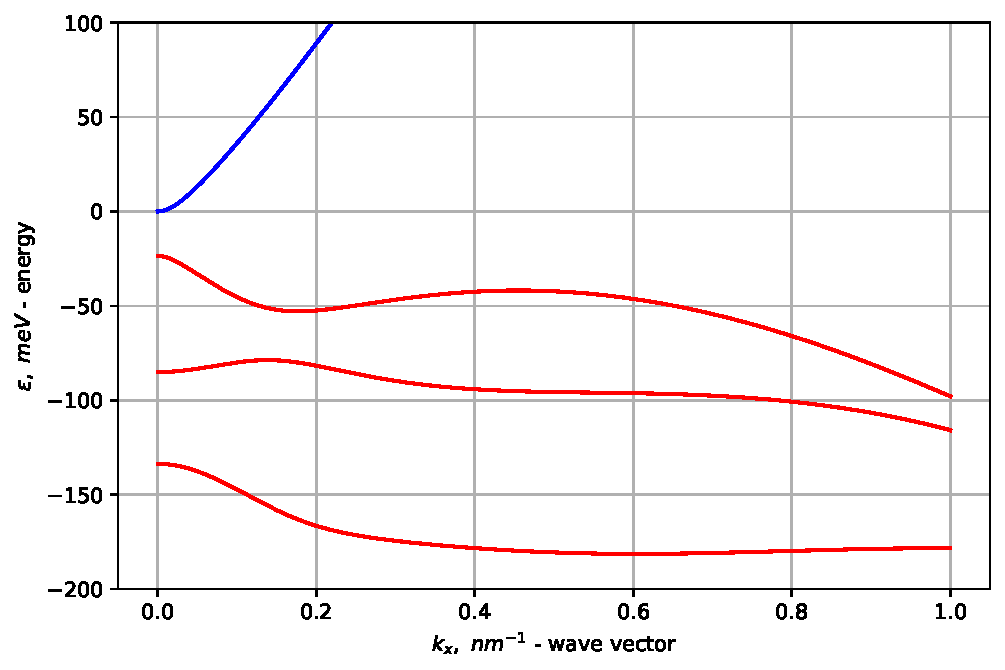
\includegraphics[width=1\textwidth]{./images/6-0-1-4.2-energy.pdf}
            \caption{Дисперсионные соотношения носителей заряда 
                                        исследуемой структуры \label{spectre}.}
        \end{minipage}
    \end{figure}

    После этого производится поиск уровней ферми для $e$ и $h$, что сводится к получению
    интегралов от вероятности нахождения частицы в точке с заданным значением спина
    и волнового вектора в зависимости от химического потенциала и решению 
    уравнения относительно $\mu$:

    \begin{equation}
        N = \sum_s \int \frac{d^2 \vec k}{1 + e^\frac{\varepsilon_s(\vec k) - \mu}{T}};
    \end{equation}

    После этого для каждого отдельно взятого значения волнового вектора плазмона 
    осуществляется поиск решения уравнений \ref{charge_full} и \ref{plasmons:disp}
    относительно $\omega \in \mathbb{C}$.

    Процесс решения является итеративным и использует одну из библиотечных функций.
    Также эта стадия крайне чувствительна к заданию начального значения. Для лучшей 
    сходимости дисперсионные соотношения полученные при близких параметрах 
    аппроксимировались полиномами и использовались в качестве начального значения для
    этой программы, что позволило существенно ускорить вычисления и уменьшить ошибки.

%ПЕРЕФОРМУЛИРОВАТЬ

    Для контроля корректности решения использовалась оценка ошибки:
    $\delta = \frac{\vec{q}^2}{2 \varepsilon \omega} \frac{2\i \sigma - c^2}{2\pi \sigma c^2}$. 
    Как пороговое решение использовалось значение $N_p$ при котором наблюдалась 
    одна точка имеющая положительное значение мнимой части частоты и которая 
    имела погрешность $\leq 10^{-3} eV$.


    \section{Результаты расчёта спектра плазмонов}

%ПОЧЕМУ ТОЛЬКО ВЕРХНЯЯ

    В дальнейшем будут показаны зонные спектры плазмонов "верхней" ветки в 
    квантовой яме толщиной $6~\text{nm}$, имеющую состав ямы $HgTe$ и 
    барьеров $CdTe$. При этом структура полагается выращенной в кристаллографическом
    направлении [013], а температура решётки и температура носителей заряда равной 
    температуре жидкого гелия $4.2~\text{K}$. Продемонстрированы срезы 
    $\vec q = (q_x, 0)$ (x по оси 100).

    \begin{figure}[h]
        \begin{minipage}[h]{0.49\textwidth}
            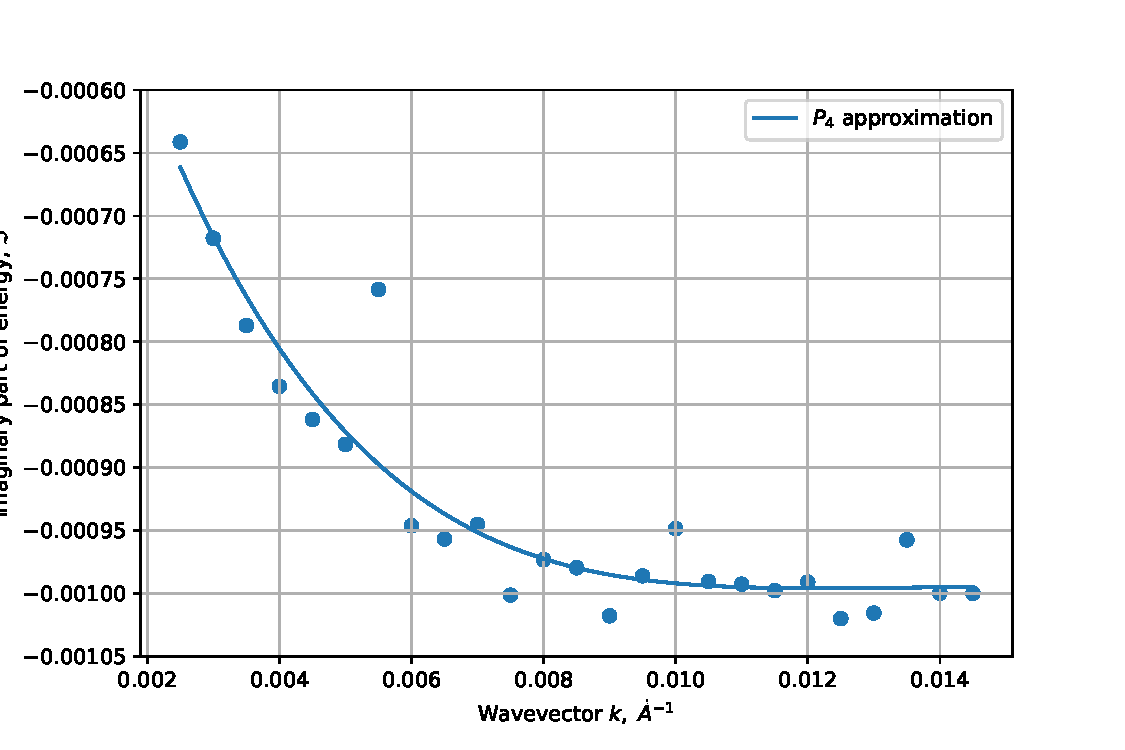
\includegraphics[width=0.9\textwidth]{./images/plasmon_6nm_25_001_im.pdf}
            \caption{Мнимая часть частоты в зависимости от волнового вектора, при $N_e = 2.5 \cdot 10^{11}~\text{cm}^{-2},~N_h = 10^9~\text{cm}^{-2}$
            \label{plasmon:6nm25ne001npim}}
        \end{minipage}
        \hfill
        \begin{minipage}[h]{0.49\textwidth}
            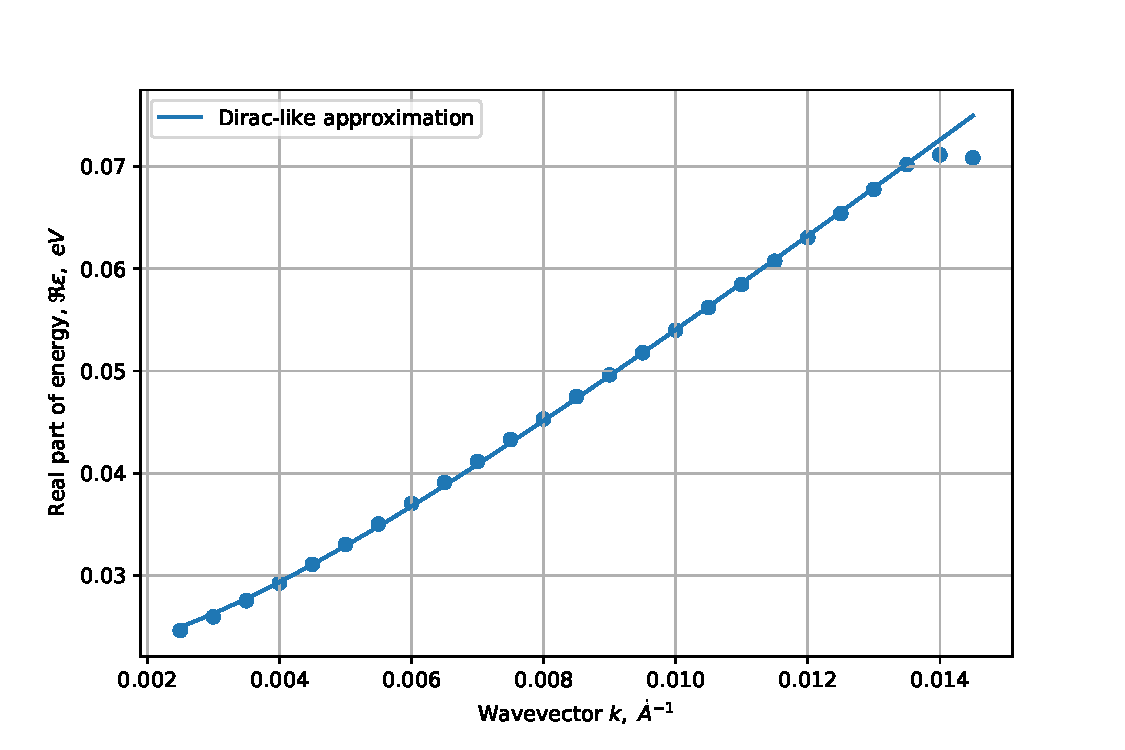
\includegraphics[width=0.9\textwidth]{./images/plasmon_6nm_25_001_re.pdf}
            \caption{Действительная часть частоты в зависимости от волнового вектора, при $N_e = 2.5 \cdot 10^{11}~\text{cm}^{-2},~N_h = 10^9~\text{cm}^{-2}$
            \label{plasmon:6nm25ne001npre}}
        \end{minipage}
    \end{figure}

    На представленных выше графиках \ref{plasmon:6nm25ne001npim}, \ref{plasmon:6nm25ne001npre} видно видно несколько особенностей.
    В частности заметно, что в данном случае плазмоны могут лишь затухать, поскольку нет достаточной инверсии населенности. 
    Также видно, что мнимая часть частоты вычисляется неустойчиво (т.е. "выбросы" на Рис. \ref{plasmon:6nm25ne001npim} 
    являются артефактами численного расчёта).

    Однако при некоторых условиях плазмоны могут иметь и положительную мнимую часть частоты, что соответствует усилению плазмонов. Для того, 
    чтобы эти условия удовлетворялись необходимо, чтобы в полупроводнике была существенная инверсия населенности, а энергия плазмона была больше 
    эффективной ширины запрещенной зоны \cite{kapralov2019feasibility}. 

    При низкой концентрации электронов энергия плазмонов будет меньше эффективной ширины запрещённой зоны. С увеличением концентрации
    равновесных носителей заряда растет и энергия плазмонов при заданном волновом векторе $\vec q$. Таким образом повышая концентрацию
    равновесных носителей можно снизить пороговую концентрацию неравновесных. 

%РАЗЖЕВАТЬ! ОБСУЖДЕНИЕ ДОБАВИТЬ
    
    Такие явления могут наблюдаться, к примеру, после накачки. 
    Особый интерес представляет "граница" концентрации, при которой будет наблюдаться усиление. Одно из таких дисперсионных соотношений 
    приведено ниже на Рис. \ref{plasmon:6nm3ne0125npim}, \ref{plasmon:6nm3ne0125npre}.

    \begin{figure}[h]
        \begin{minipage}[h]{0.49\textwidth}
            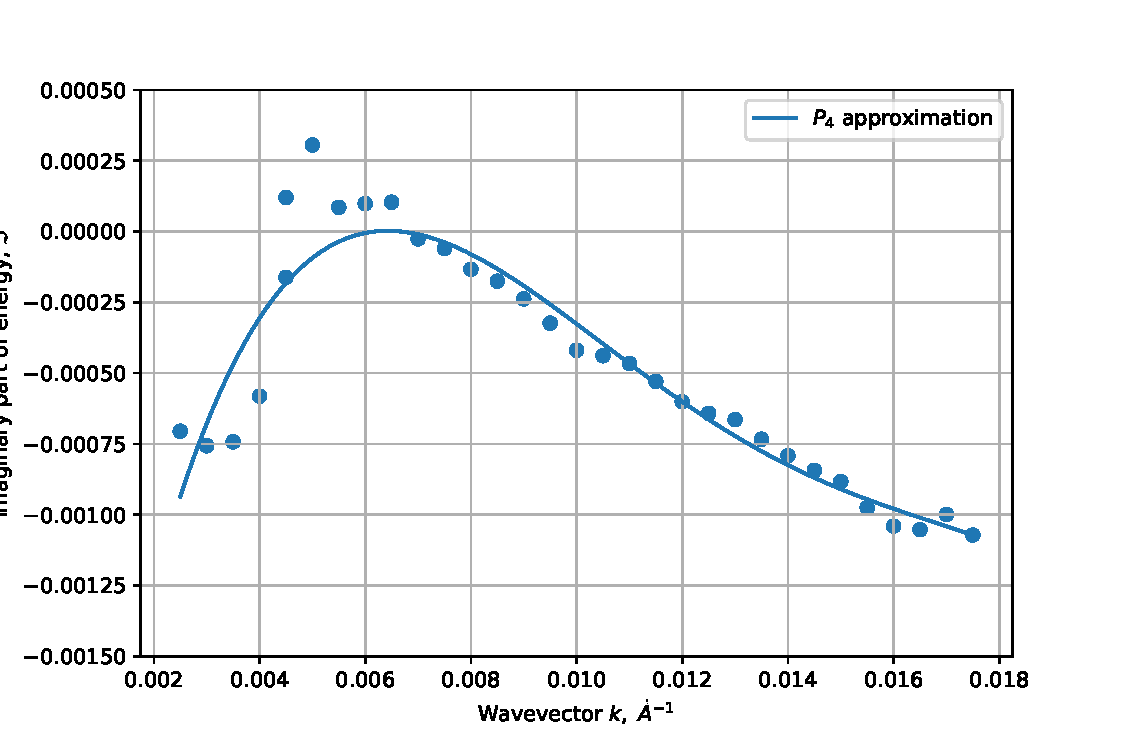
\includegraphics[width=0.9\textwidth]{./images/plasmon_6nm_3_0125_im.pdf}
            \caption{Мнимая часть частоты в зависимости от волнового вектора, при $N_e = 3 \cdot 10^{11}~\text{cm}^{-2},~N_h = 1.25 \cdot 10^{10}~\text{cm}^{-2}$
            \label{plasmon:6nm3ne0125npim}}
        \end{minipage}
        \hfill
        \begin{minipage}[h]{0.49\textwidth}
            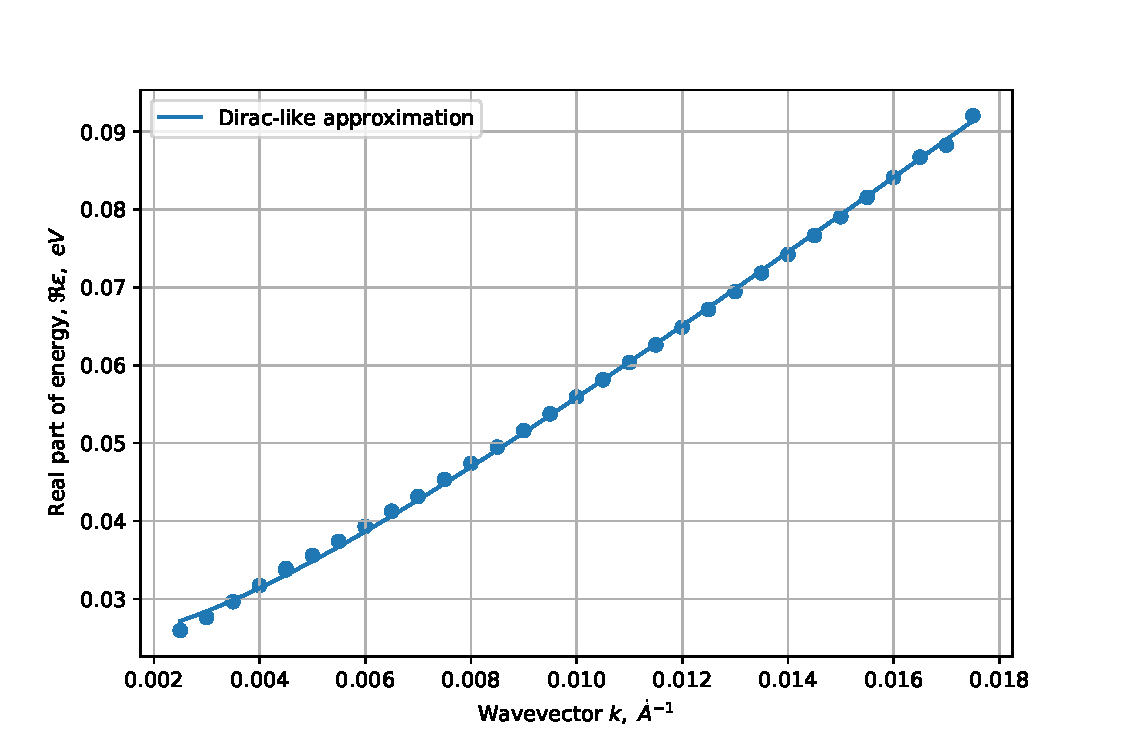
\includegraphics[width=0.9\textwidth]{./images/plasmon_6nm_3_0125_re.pdf}
            \caption{Действительная часть частоты в зависимости от волнового вектора, при $N_e = 3 \cdot 10^{11}~\text{cm}^{-2},~N_h = 1.25 \cdot 10^{10}~\text{cm}^{-2}$
            \label{plasmon:6nm3ne0125npre}}
        \end{minipage}
    \end{figure}

    Для того чтобы оценить, что действительно существует порог можно посмотреть на сводную диаграмму для семейства зависимостей $\Im \omega(\vec q)$
    (мнимой части дисперсионных соотношений) при постоянной концентрации электронов и изменяющейся концентрации дырок \ref{plasmon:6nm3neXnpim}.
    Стоит отметить, что именно эта зависимость определяет коэффициент усиления/поглощения:
    \begin{equation}
        \alpha(\Re \omega (\vec q)) = -2 \Im \omega \Re \left(\frac{d\omega}{d\vec q}\right)^{-1};
    \end{equation}

    \begin{figure}[h]
        \begin{minipage}[h]{1\textwidth}
            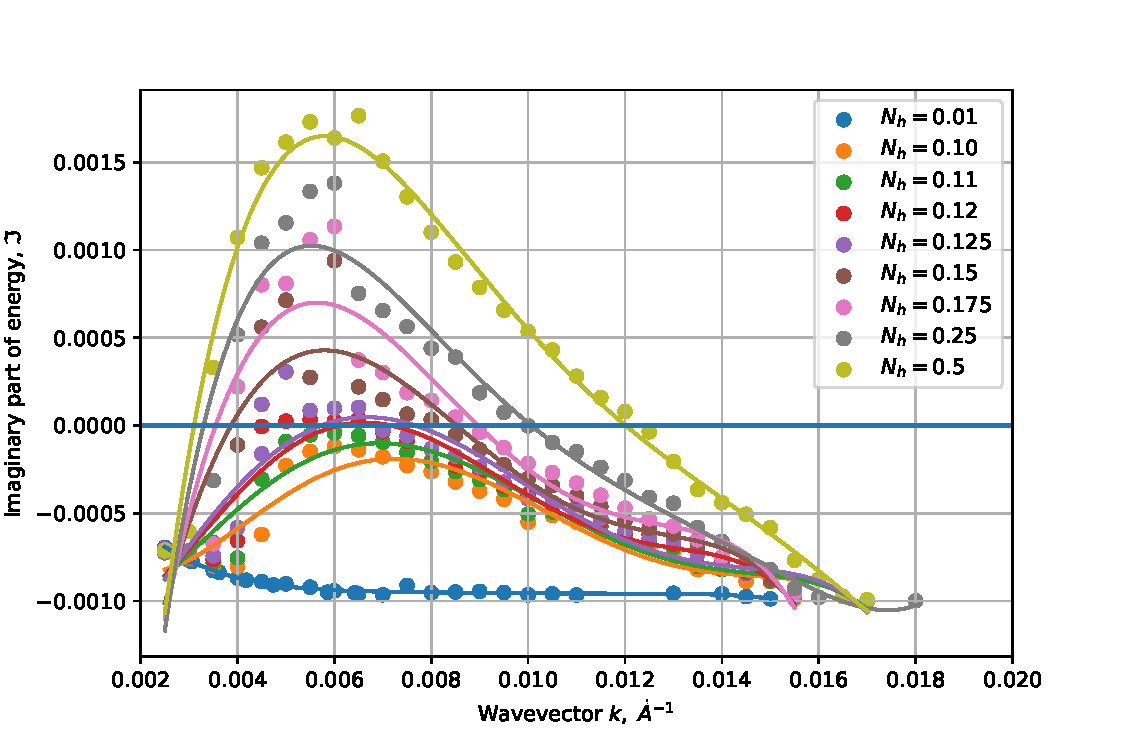
\includegraphics[width=1\textwidth]{./images/plazmon6nm3neXnpim.pdf}
            \caption{Мнимая часть частоты в зависимости от волнового вектора, при 
            $N_e = 3 \cdot 10^{11}~\text{cm}^{-2},~N_h = x \cdot 10^{10}~\text{cm}^{-2}$,
            где $x$ указан на графике.\label{plasmon:6nm3neXnpim}}
        \end{minipage}
    \end{figure}

    \section{Пороговая неравновесная концентрация усиления}

    Важным возможным применением подобных структур является усиление ЭМ волн. 
    Коэффициент усиления, однако, не всегда является положительным и 
    зависит от волнового вектора плазмона $\omega(\vec q)$, 
    а также от параметров структуры - равновесной и индуцированной 
    (например легированием) концентрации носителей. 

    Очевидно, что чем меньше равновесная концентрация - тем 
    сложнее добиться усиления, т.к. меньше и инверсия населенностей.

%РАСПИСАТЬ ПОДРОБНЕЕ 

    \begin{figure}[h]
        \begin{minipage}[h]{1\textwidth}
            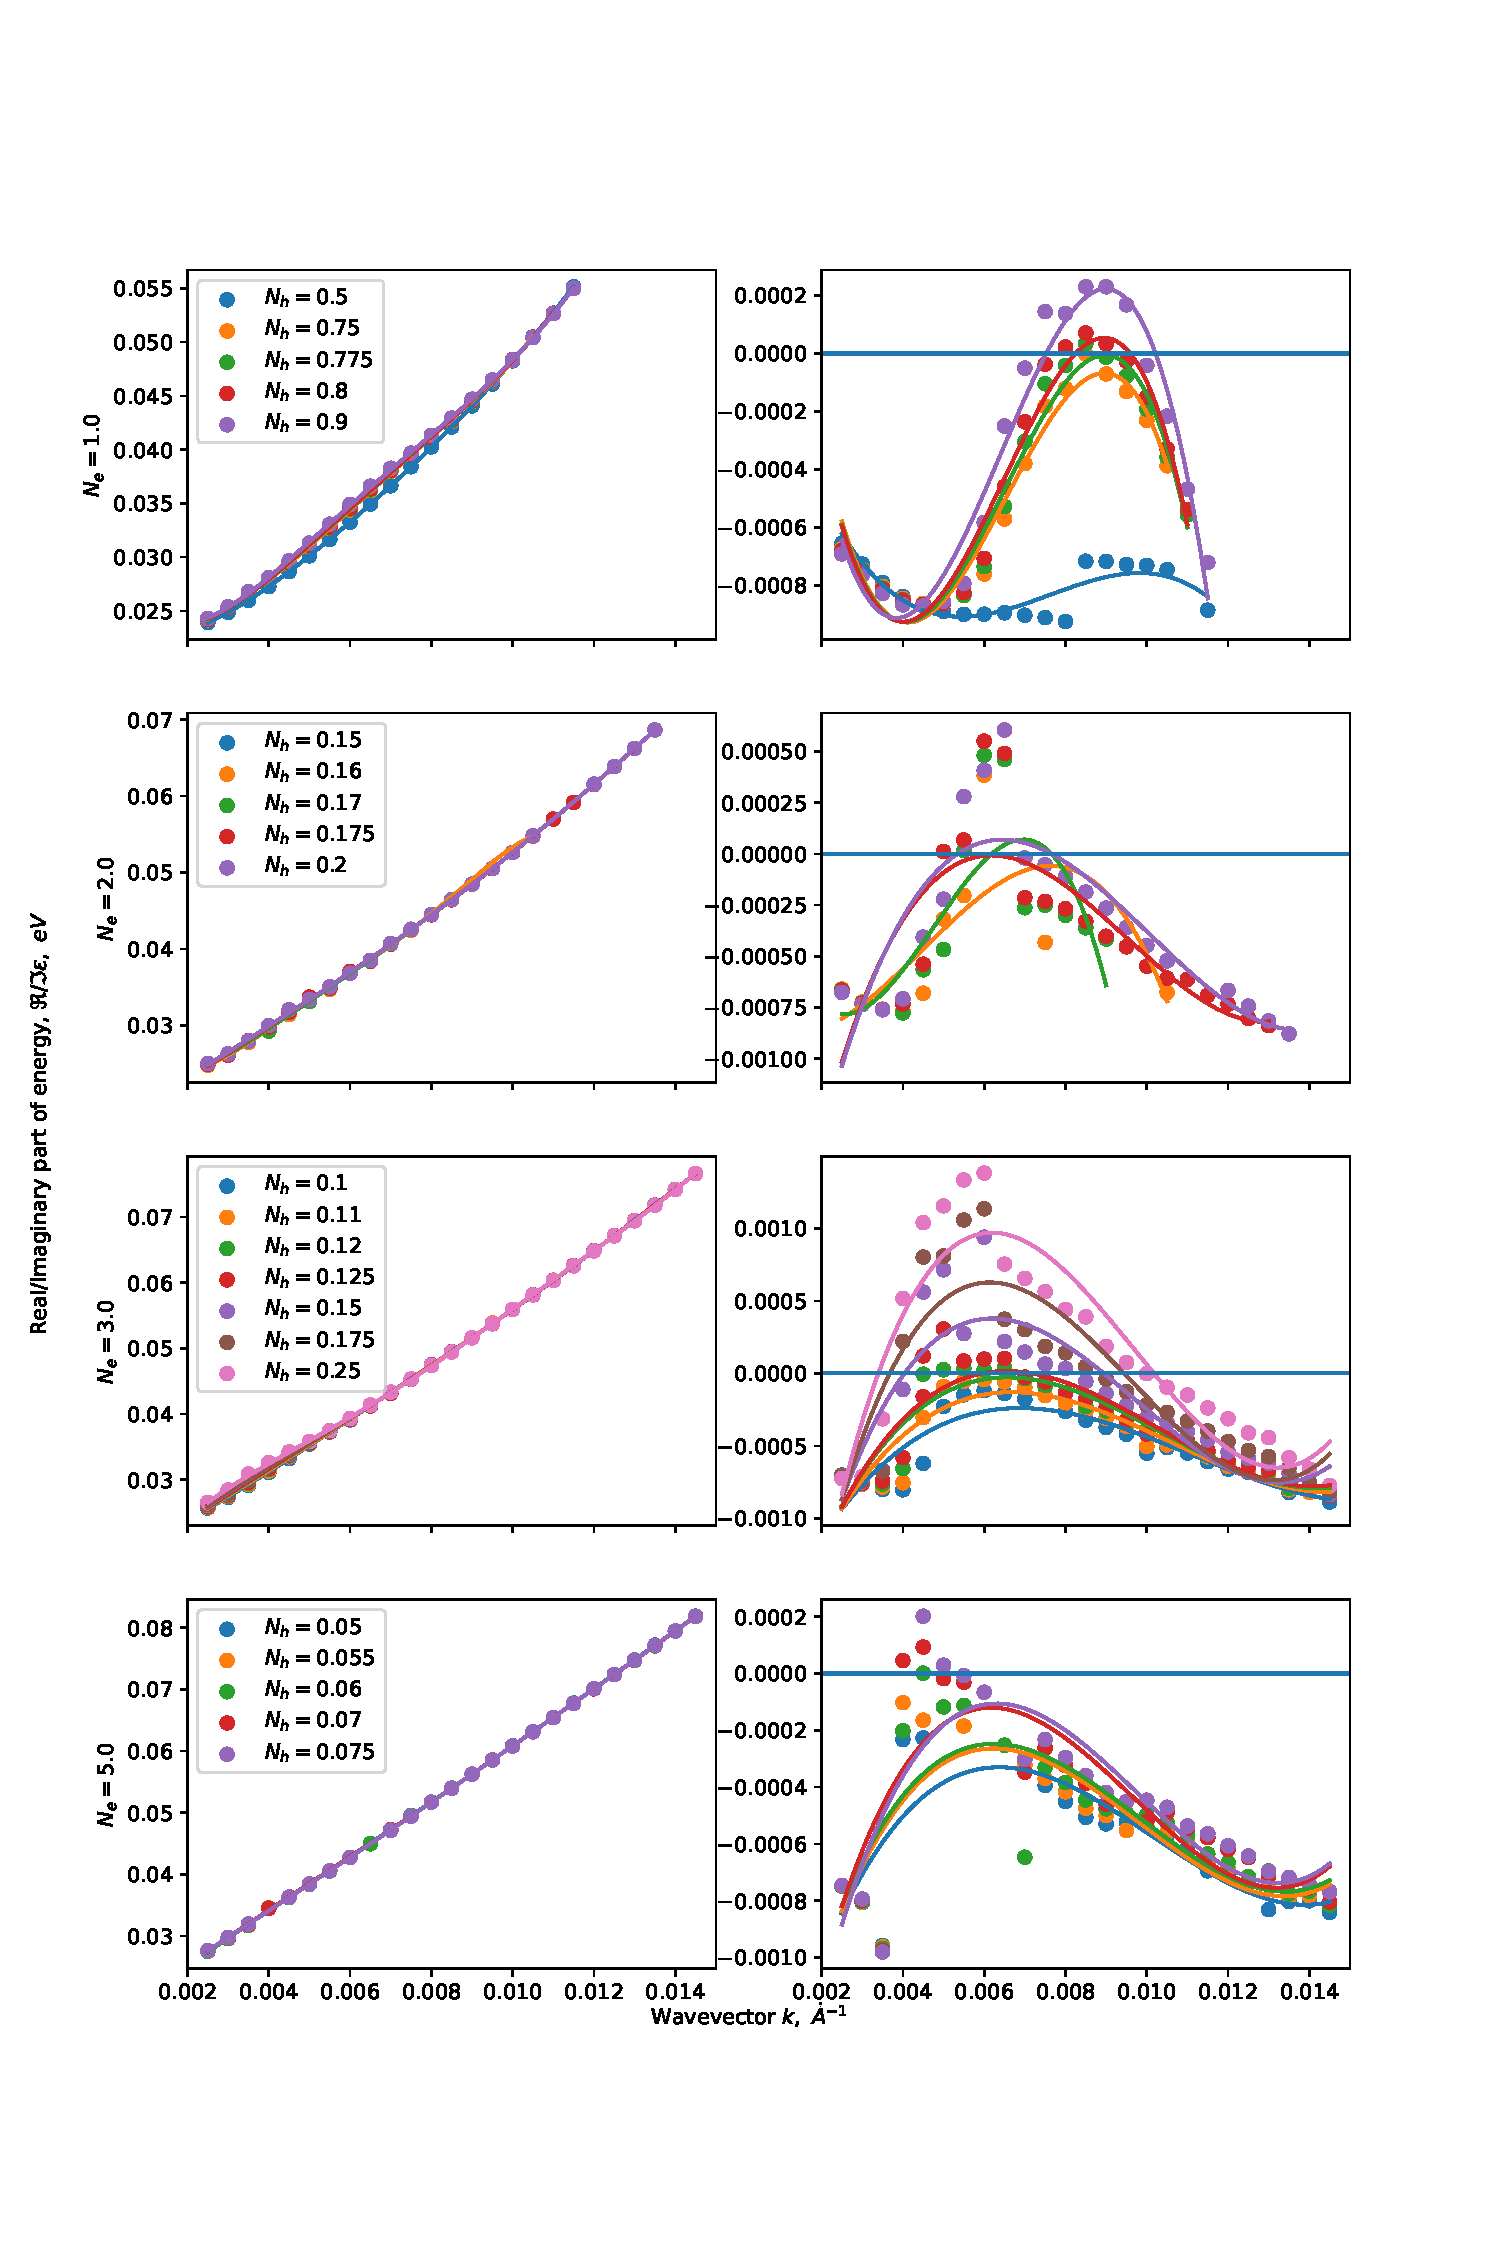
\includegraphics[width=1\textwidth]{./images/compare_plots_6nm_42K.pdf}
            \caption{Дисперсионные соотношения плазмонов, при разных концентрациях 
            носителей. \label{plasmon:compare_42}
            Концентрации указаны в $\cdot 10^{11} \text{cm}^{-2}$.}
        \end{minipage}
    \end{figure}

    Таким образом была получена зависимость пороговой концентрации дырок 
    $N_h$ от концентрации электронов $N_e$. Она представлена ниже:

    \begin{figure}[h]
        \begin{minipage}[h]{1\textwidth}
            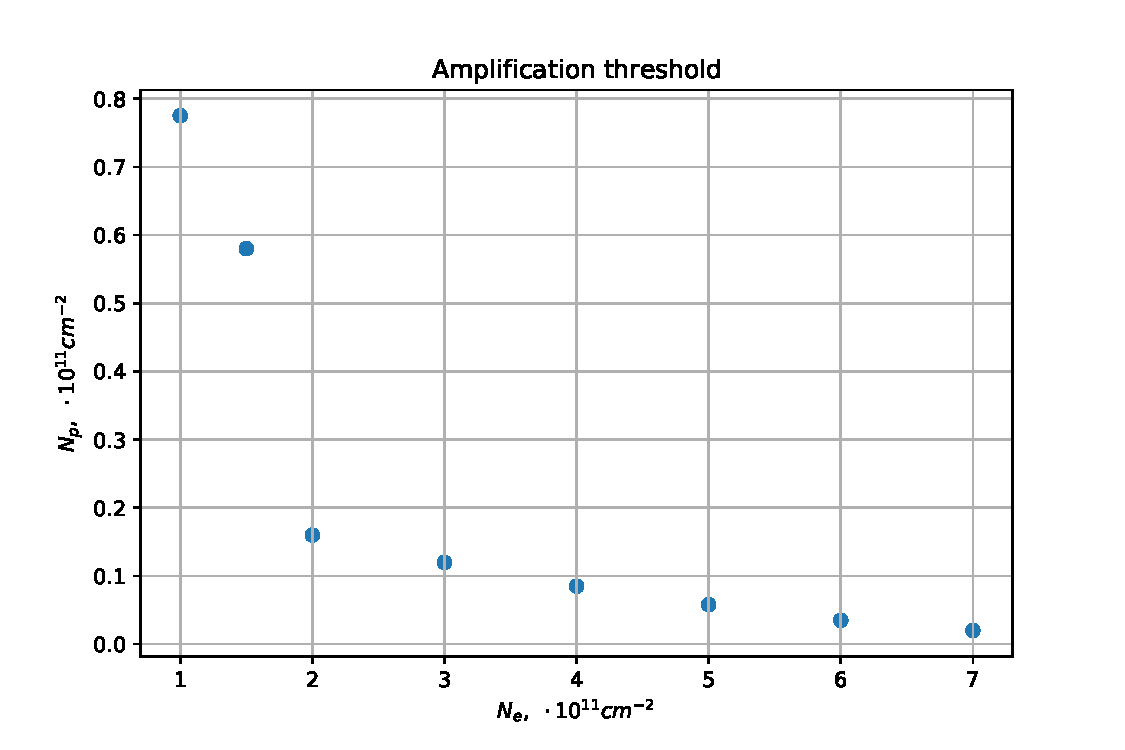
\includegraphics[width=1\textwidth]{./images/threshold_6nm_42K.pdf}
            \caption{Пороговые концентрации носителей \label{plasmon:threshold_42}.}
        \end{minipage}
    \end{figure}

\end{document}